\chapter[Analise dos Resultados]{Analise dos Resultados e Discussões}
\addcontentsline{toc}{chapter}{analise dos Resultados e discussões}
\label{chap:analiseResultados}

Este capítulo apresenta a análise dos resultados obtidos com a execução dos modelos de treinamento centralizado e distribuído. Além disso, é exposta a análise do autor referente aos dados coletados e as impressões obtidas durante a execução dos experimentos. Confere-se, inicialmente há a apresentação dos resultados obtidos, acompanhada pela \hyperref{sec:resultados}{Análise dos Resultados}. Posteriormente, são discutidas as dificuldades e limitações encontradas durante a execução dos experimentos.

Serão apresentados e discutidos os desempenhos dos modelos desenvolvidos ao longo do projeto, tanto no contexto centralizado quanto no federado. Três modelos centralizados foram implementados: uma rede neural convolucional (CNN), uma rede neural multicamadas (MLP) e uma rede neural profunda (DNN). Esses modelos serão comparados com o modelo de aprendizado federado, permitindo uma análise detalhada das métricas obtidas, como acurácia, precisão, recall, F1-score e o tempo de processamento. A comparação entre os modelos visa identificar as vantagens e limitações de cada abordagem, destacando o impacto do aprendizado federado na preservação de privacidade dos dados e na eficiência do treinamento distribuído.

\section{Análise dos Resultados}
\label{sec:resultados}

\section{Desempenho dos Modelos Centralizados}

\subsection{Modelo Centralizado - Rede neural convolucional}

Um dos modelos centralizados foi implementado utilizando uma rede neural convolucional (CNN) e treinado sobre o conjunto de dados MNIST. Este modelo foi configurado para realizar cinco épocas de treinamento, com um tamanho de lote de 32, utilizando o otimizador Adam e a função de perda \texttt{sparse\_categorical\_crossentropy}. Durante o processo, as métricas de acurácia e perda foram acompanhadas tanto no conjunto de treinamento quanto no de validação, permitindo uma análise detalhada do comportamento do modelo ao longo das épocas.

\begin{figure}[ht]
    \centering
    \caption{Curvas de acurácia do modelo centralizado - CNN}
    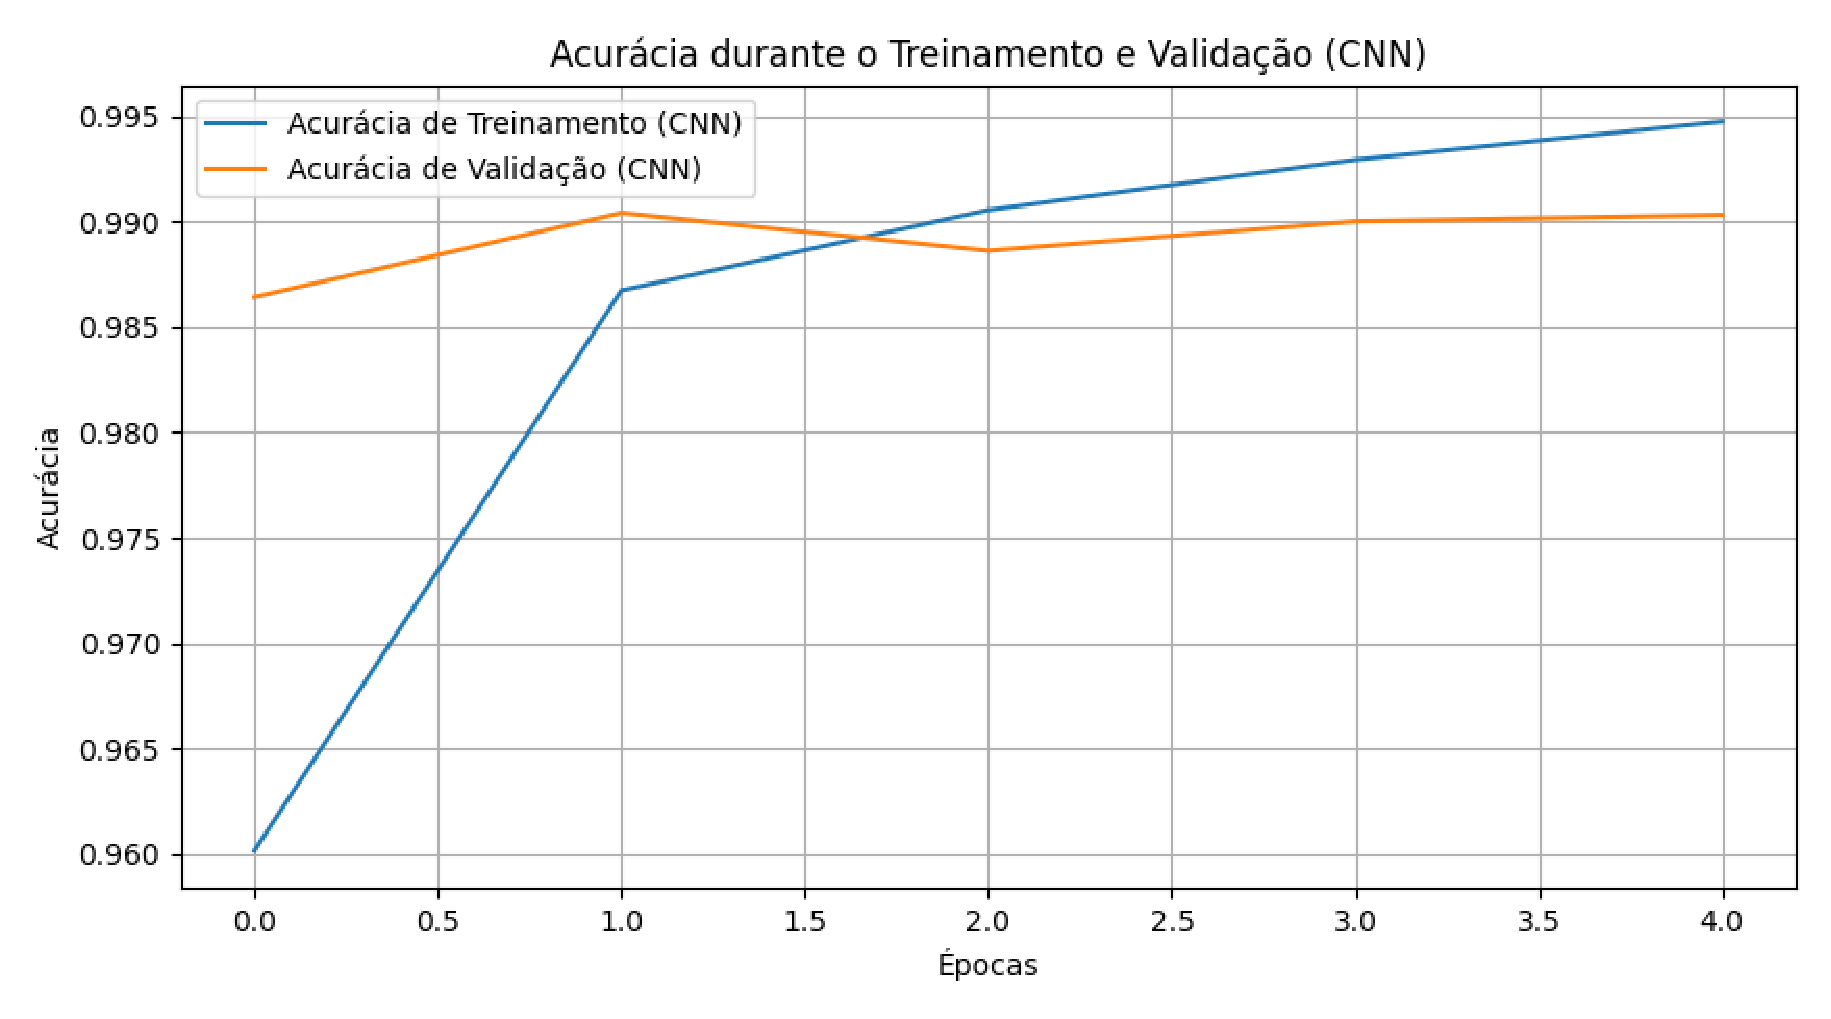
\includegraphics[scale=0.4]{figuras/analiseResultados/acuracyCNN.eps}
    \label{fig:acuracyCNN}
    \fonte{Elaborado pelo autor.}
\end{figure}

Os resultados obtidos indicam um desempenho satisfatório do modelo centralizado. A acurácia no conjunto de teste alcançou 99,03\%, com uma perda de 0,0302, o que evidencia a capacidade do modelo de generalizar para dados não vistos. Além disso, o tempo total de treinamento foi de 337,32 segundos (aproximadamente 5 minutos e 37 segundos), o que demonstra uma eficiência razoável, dada a complexidade do modelo e o tamanho do conjunto de dados.

\begin{figure}[ht]
    \centering
    \caption{Curvas de perda do modelo centralizado - CNN}
    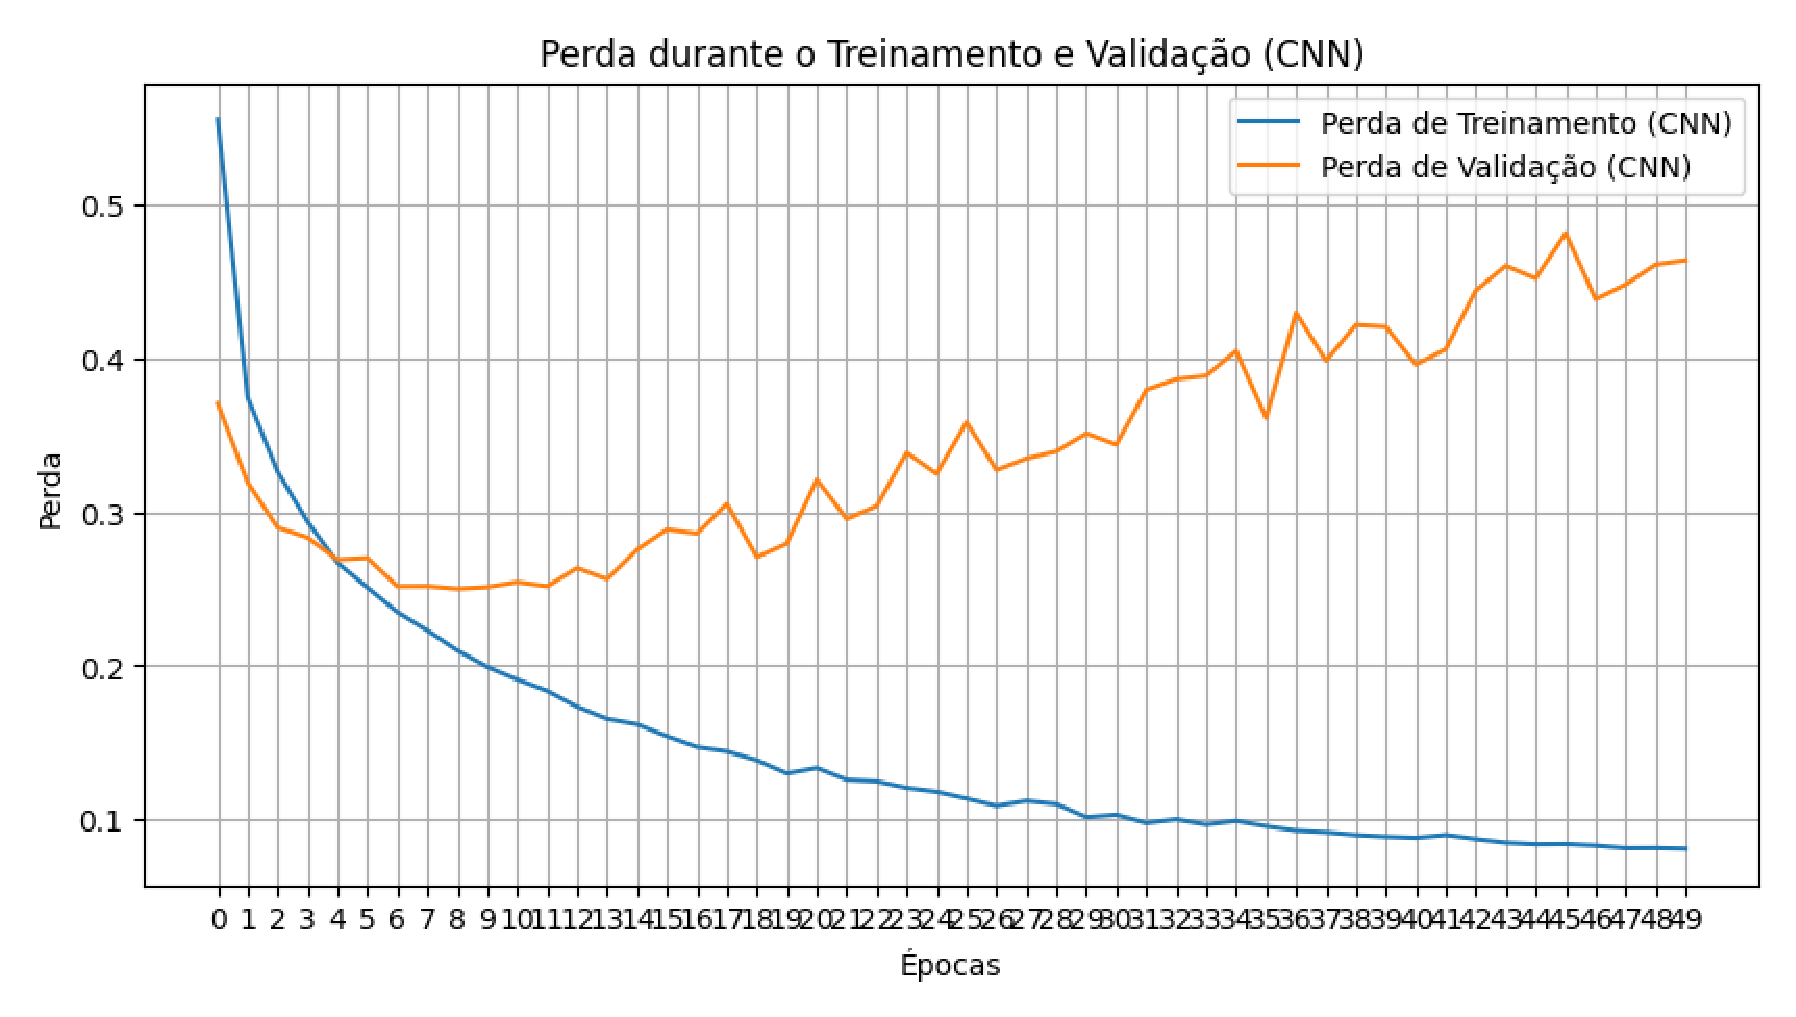
\includegraphics[scale=0.4]{figuras/analiseResultados/lossCNN.eps}
    \label{fig:lossCNN}
    \fonte{Elaborado pelo autor.}
\end{figure}

Durante o treinamento, observou-se uma melhoria constante na acurácia, tanto no conjunto de treinamento quanto no de validação, atingindo valores próximos de 99\% já na segunda época. Essa tendência continuou ao longo das épocas subsequentes, com uma pequena oscilação nos valores de perda, mas sem indícios de \textit{overfitting}, dado que as curvas de acurácia e perda de validação acompanharam de perto as de treinamento.

\subsection{Modelo Centralizado - Rede neural multicamadas}

O modelo centralizado apresentado nesta seção foi desenvolvido utilizando uma Rede Neural Multicamadas (MLP), composta por quatro camadas densas, das quais três utilizam a função de ativação ReLU e a camada de saída utiliza a função \textit{softmax} para classificação. O objetivo deste modelo é classificar as imagens da base de dados MNIST, que foram achatadas para uma dimensão de 28x28, correspondendo a 784 entradas para cada amostra.

\begin{figure}[ht]
    \centering
    \caption{Curvas de acurácia do modelo centralizado - MLP}
    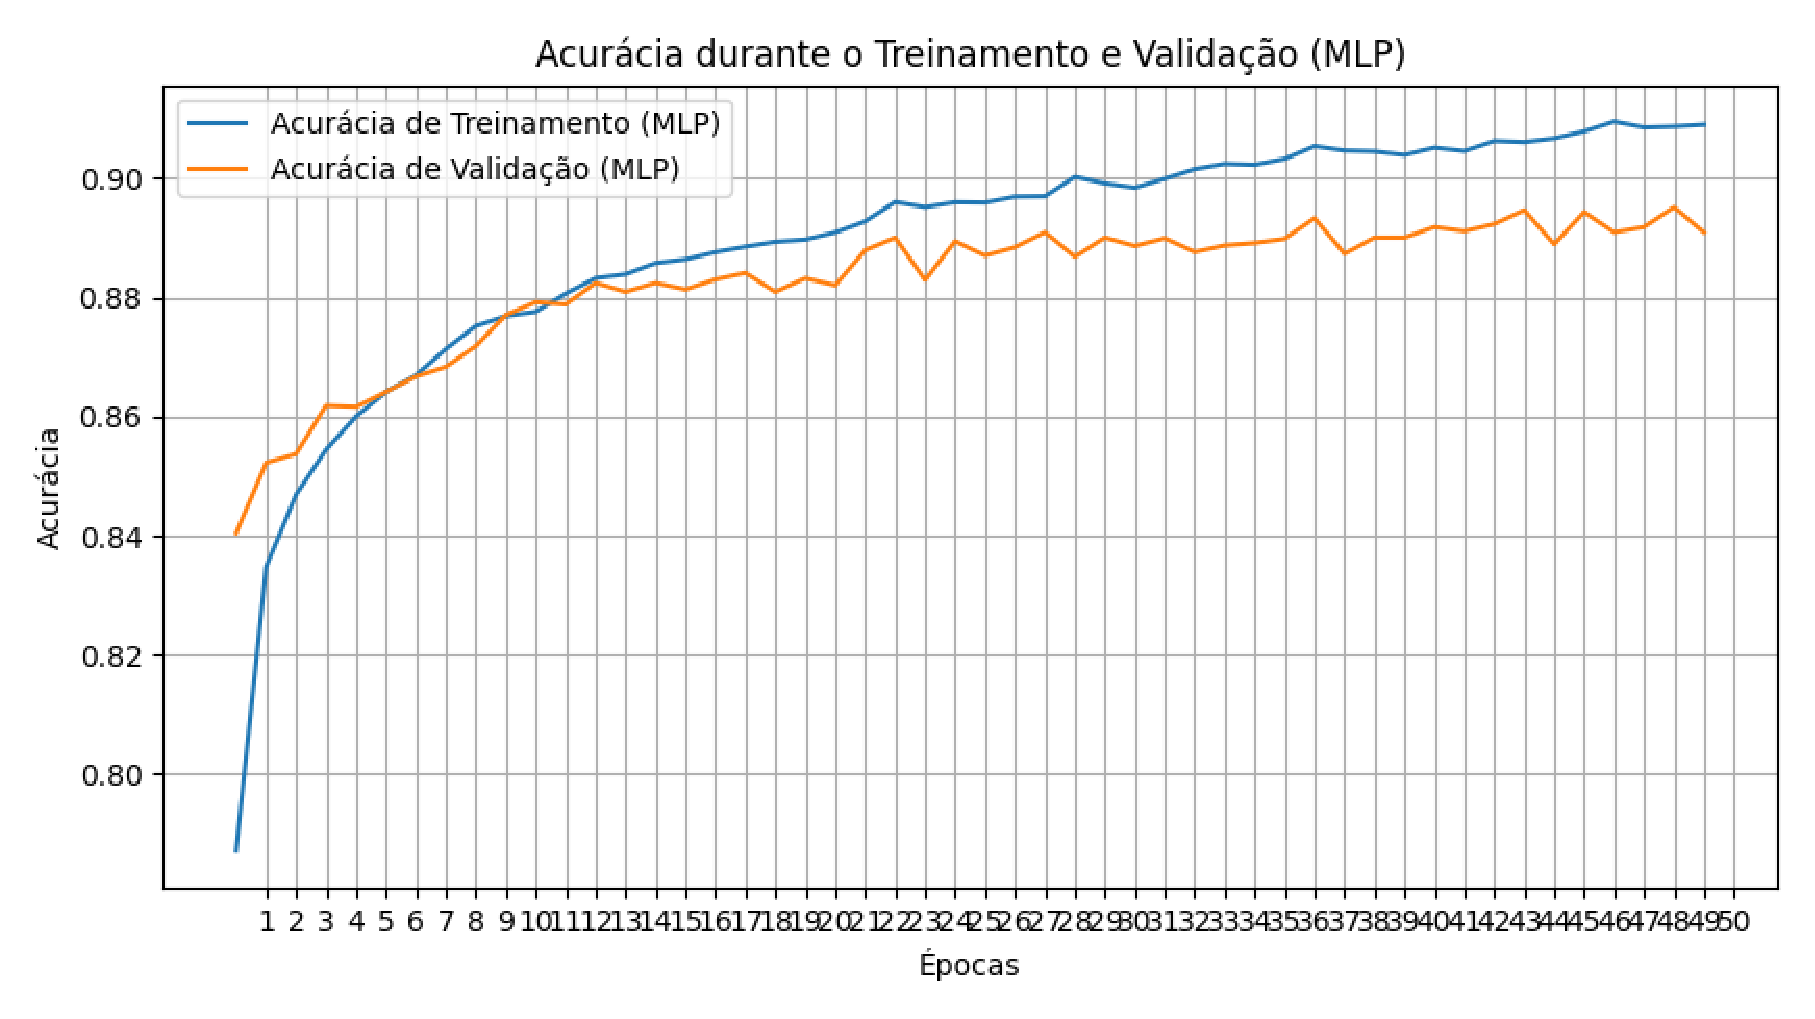
\includegraphics[scale=0.4]{figuras/analiseResultados/acuracyMLP.eps}
    \label{fig:acuracyMLP}
    \fonte{Elaborado pelo autor.}
\end{figure}

Após o treinamento do modelo por 5 épocas, com um tamanho de \textit{batch} de 32, foi possível observar um desempenho consistente. A acurácia de treinamento evoluiu de 89,36\% na primeira época para 98,88\% na quinta. Nos dados de validação, o modelo apresentou uma acurácia de 96,87\% já na primeira época, atingindo 97,67\% ao final do treinamento. Esse resultado demonstra a capacidade do MLP de generalizar bem para dados não vistos, o que se reflete no desempenho ao testar o modelo com dados de teste, onde obteve uma acurácia de 97,34\%.

\begin{figure}[ht]
    \centering
    \caption{Curvas de perda do modelo centralizado - MLP}
    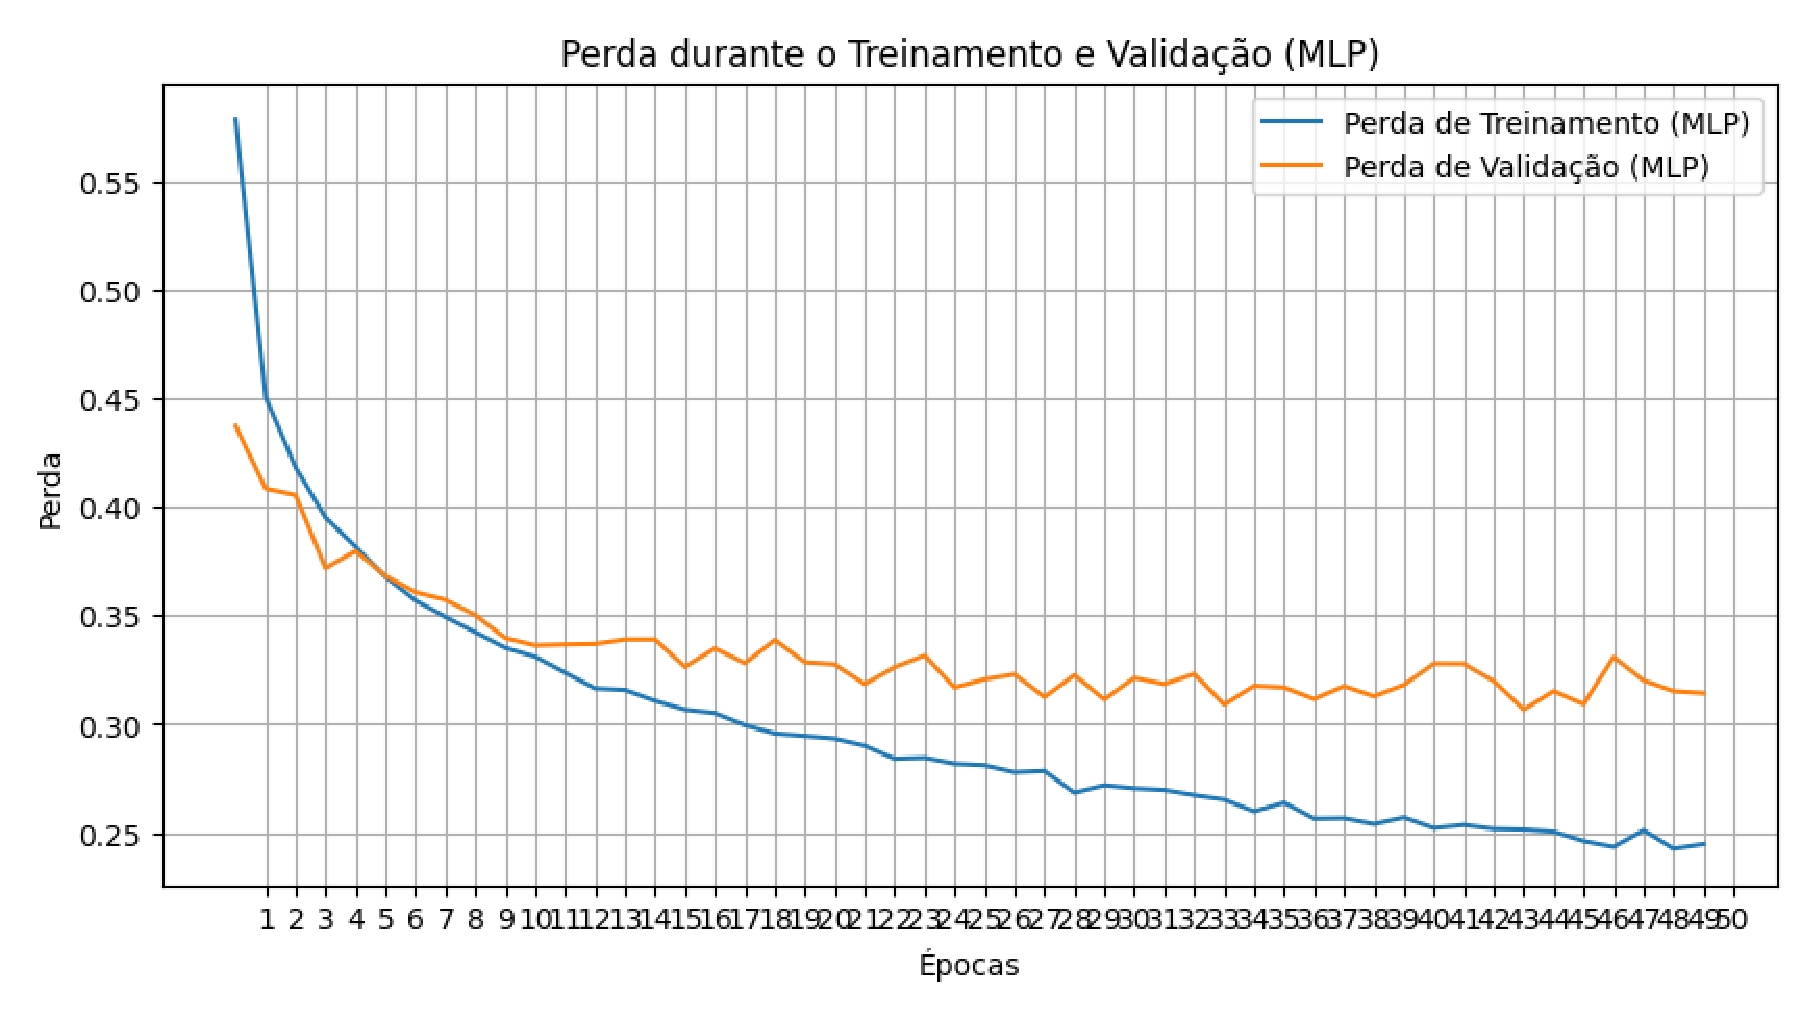
\includegraphics[scale=0.4]{figuras/analiseResultados/lossMLP.eps}
    \label{fig:lossMLP}
    \fonte{Elaborado pelo autor.}
\end{figure}

Em termos de perda, o modelo começou com um valor de 0,3457 na primeira época, reduzindo para 0,0346 na última, o que indica uma boa otimização do erro durante o treinamento. A perda nos dados de validação seguiu uma trajetória estável, permanecendo em torno de 0,0856 ao final do processo, sugerindo que o modelo conseguiu evitar o \textit{overfitting}, uma vez que as métricas de validação e treinamento se mantiveram próximas.

O tempo total de treinamento foi de aproximadamente 114 segundos, o que representa um tempo relativamente rápido para o conjunto de dados MNIST, considerando a arquitetura utilizada. Esse desempenho do MLP indica que redes densas profundas podem ser eficazes na resolução de problemas de classificação de imagens simples como o MNIST, mas também evidencia a necessidade de modelos mais avançados para melhorar ainda mais a precisão e o tempo de treinamento, comparando, por exemplo, com redes convolucionais (CNNs).

\subsection{Modelo Centralizado - Rede neural profunda}

Nesta seção, é analisado o desempenho de um modelo centralizado desenvolvido utilizando uma Rede Neural Profunda (DNN). O modelo foi composto por cinco camadas densas, sendo quatro com a função de ativação ReLU e uma camada de saída com a função \textit{softmax}, projetada para realizar a classificação das imagens da base de dados MNIST.

Durante o treinamento, que foi realizado em 5 épocas com um tamanho de \textit{batch} de 32, o modelo apresentou uma acurácia de 89,85\% já na primeira época, chegando a 98,75\% ao final. A acurácia de validação também foi expressiva, alcançando 95,52\% na primeira época e 97,60\% na última. Esses resultados demonstram uma boa capacidade de generalização do modelo, mesmo ao trabalhar com dados não vistos.

\begin{figure}[ht]
    \centering
    \caption{Curvas de acurácia do modelo centralizado - DNN}
    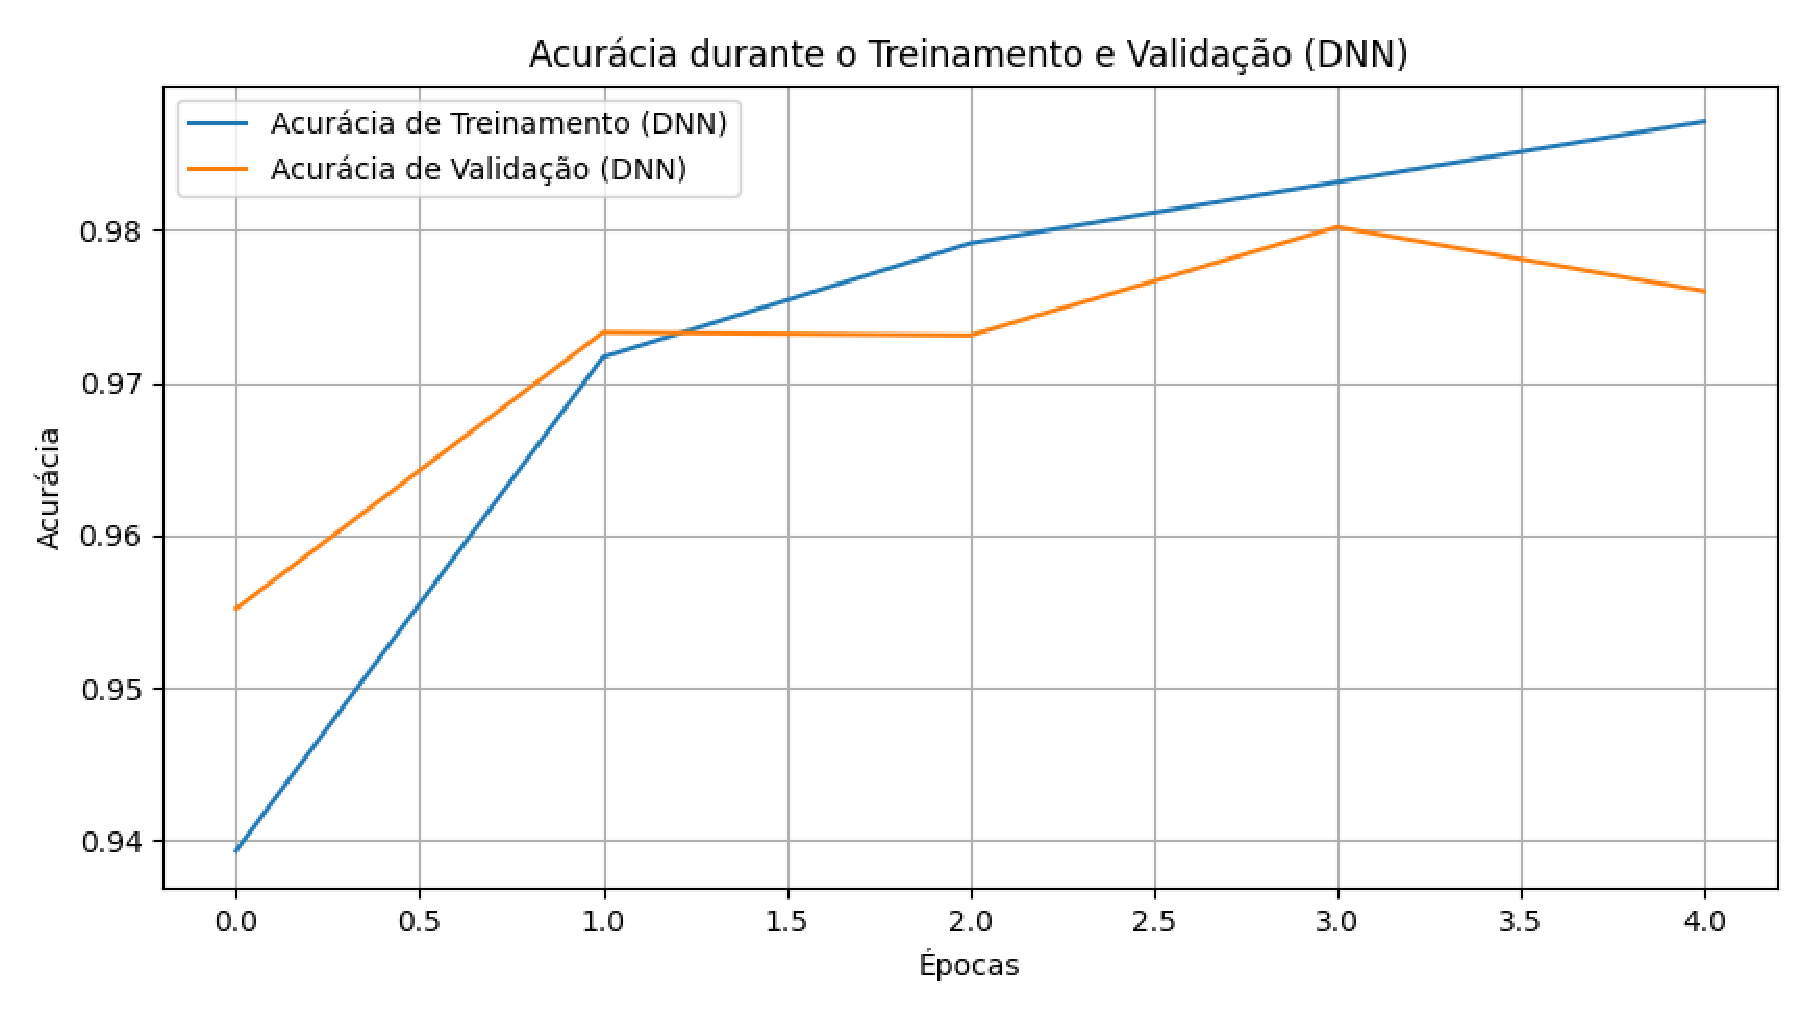
\includegraphics[scale=0.4]{figuras/analiseResultados/acuracyDNN.eps}
    \label{fig:acuracyDNN}
    \fonte{Elaborado pelo autor.}
\end{figure}

A análise da perda durante o treinamento e validação reflete uma trajetória semelhante. Inicialmente, o modelo apresentou uma perda de 0,3233, que foi reduzida para 0,0404 ao final do processo de treinamento. Nos dados de validação, a perda começou em 0,1489 e chegou a 0,0975, sugerindo que o modelo conseguiu manter um bom equilíbrio entre a minimização do erro e a generalização, sem indícios de \textit{overfitting} significativos.

\begin{figure}[ht]
    \centering
    \caption{Curvas de perda do modelo centralizado - DNN}
    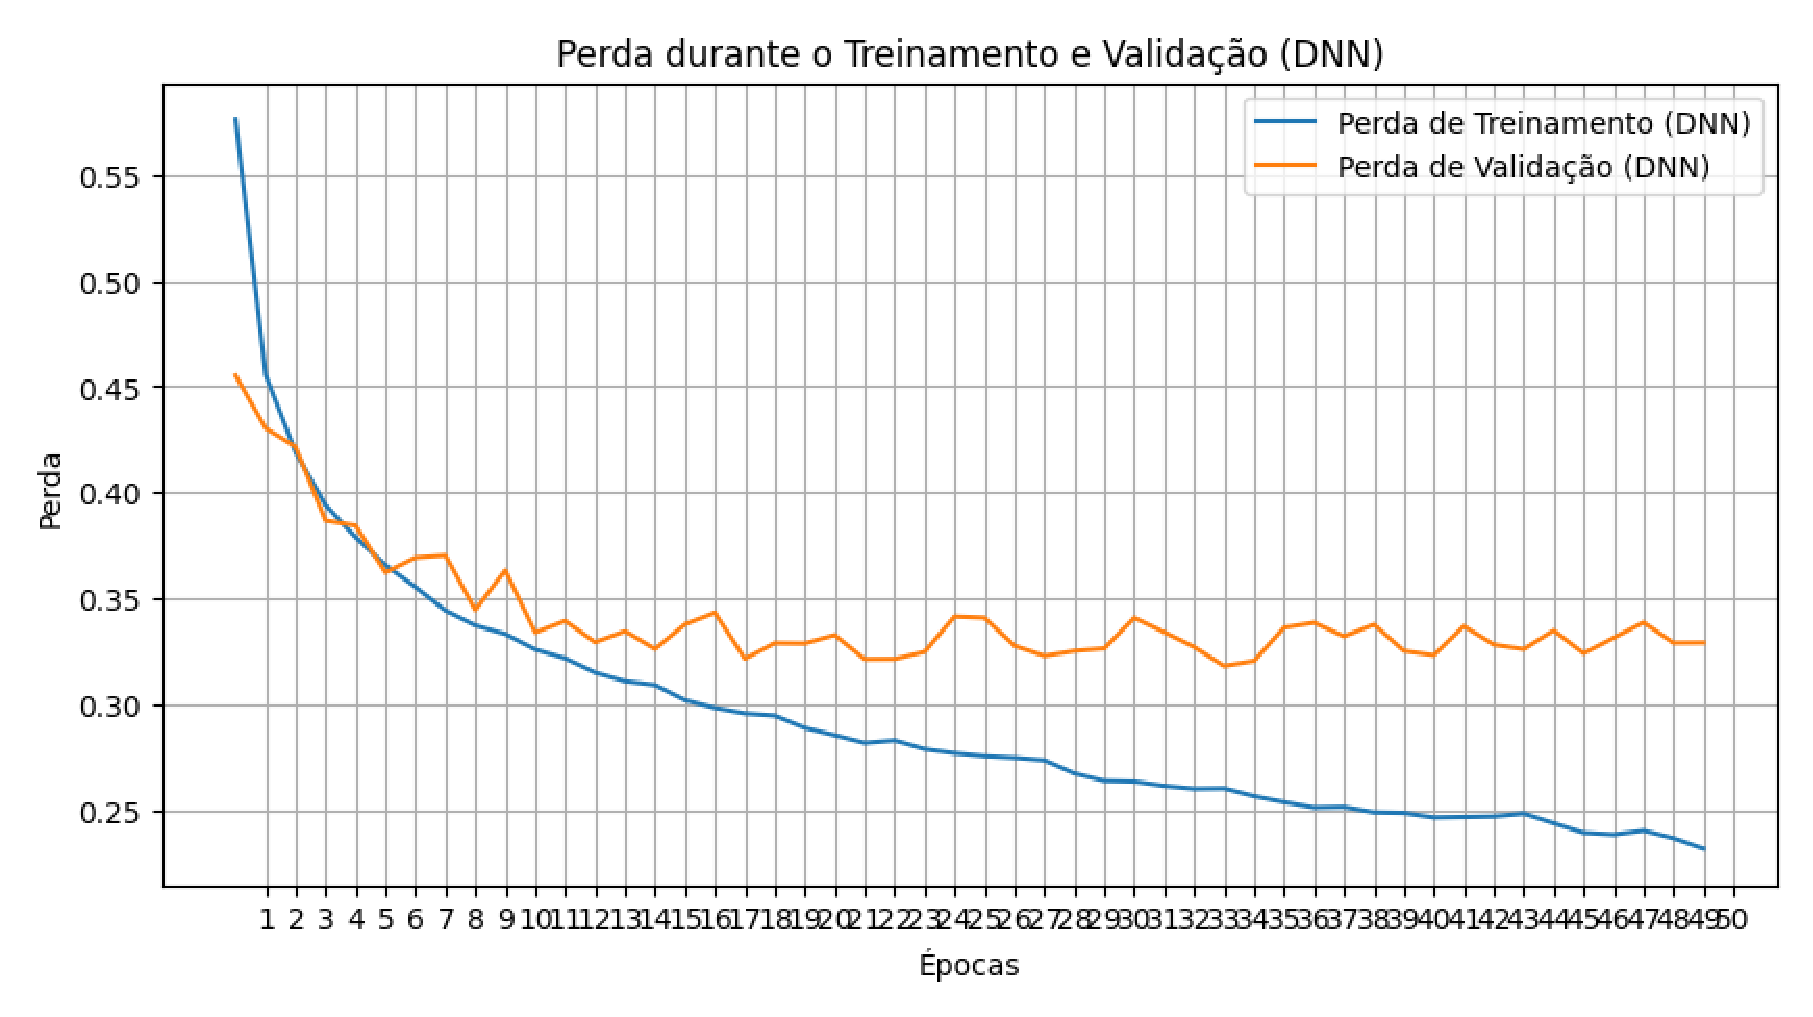
\includegraphics[scale=0.4]{figuras/analiseResultados/lossDNN.eps}
    \label{fig:lossDNN}
    \fonte{Elaborado pelo autor.}
\end{figure}

Ao testar o modelo com dados de teste, a acurácia obtida foi de 97,30\%, o que demonstra uma consistência com os resultados de validação. O tempo total de treinamento foi de aproximadamente 318 segundos, um aumento considerável em relação ao modelo MLP, o que reflete a maior complexidade e o número de parâmetros do DNN.

Esse desempenho destaca o potencial do DNN em tarefas de classificação mais complexas, como a classificação de imagens, quando comparado a modelos mais simples. A análise comparativa com outros modelos centralizados, como a CNN e a MLP, será realizada para avaliar a relação entre o tempo de processamento e a precisão obtida.

\section{Resultados do Modelo Federado}

Nesta seção, é analisado o desempenho de um modelo federado utilizando a abordagem de aprendizado federado com o algoritmo de \textit{FedAvg}. O modelo foi projetado com uma arquitetura de rede neural convolucional (CNN) para classificar as imagens da base de dados MNIST. O treinamento federado foi realizado por 10 rodadas, distribuindo os dados entre 10 clientes, utilizando as métricas de acurácia categórica esparsa e acurácia \textit{Top-3}.

\subsection{Acurácia por Rodada}

\begin{figure}[ht]
    \centering
    \caption{Curvas de acurácia do modelo federado}
    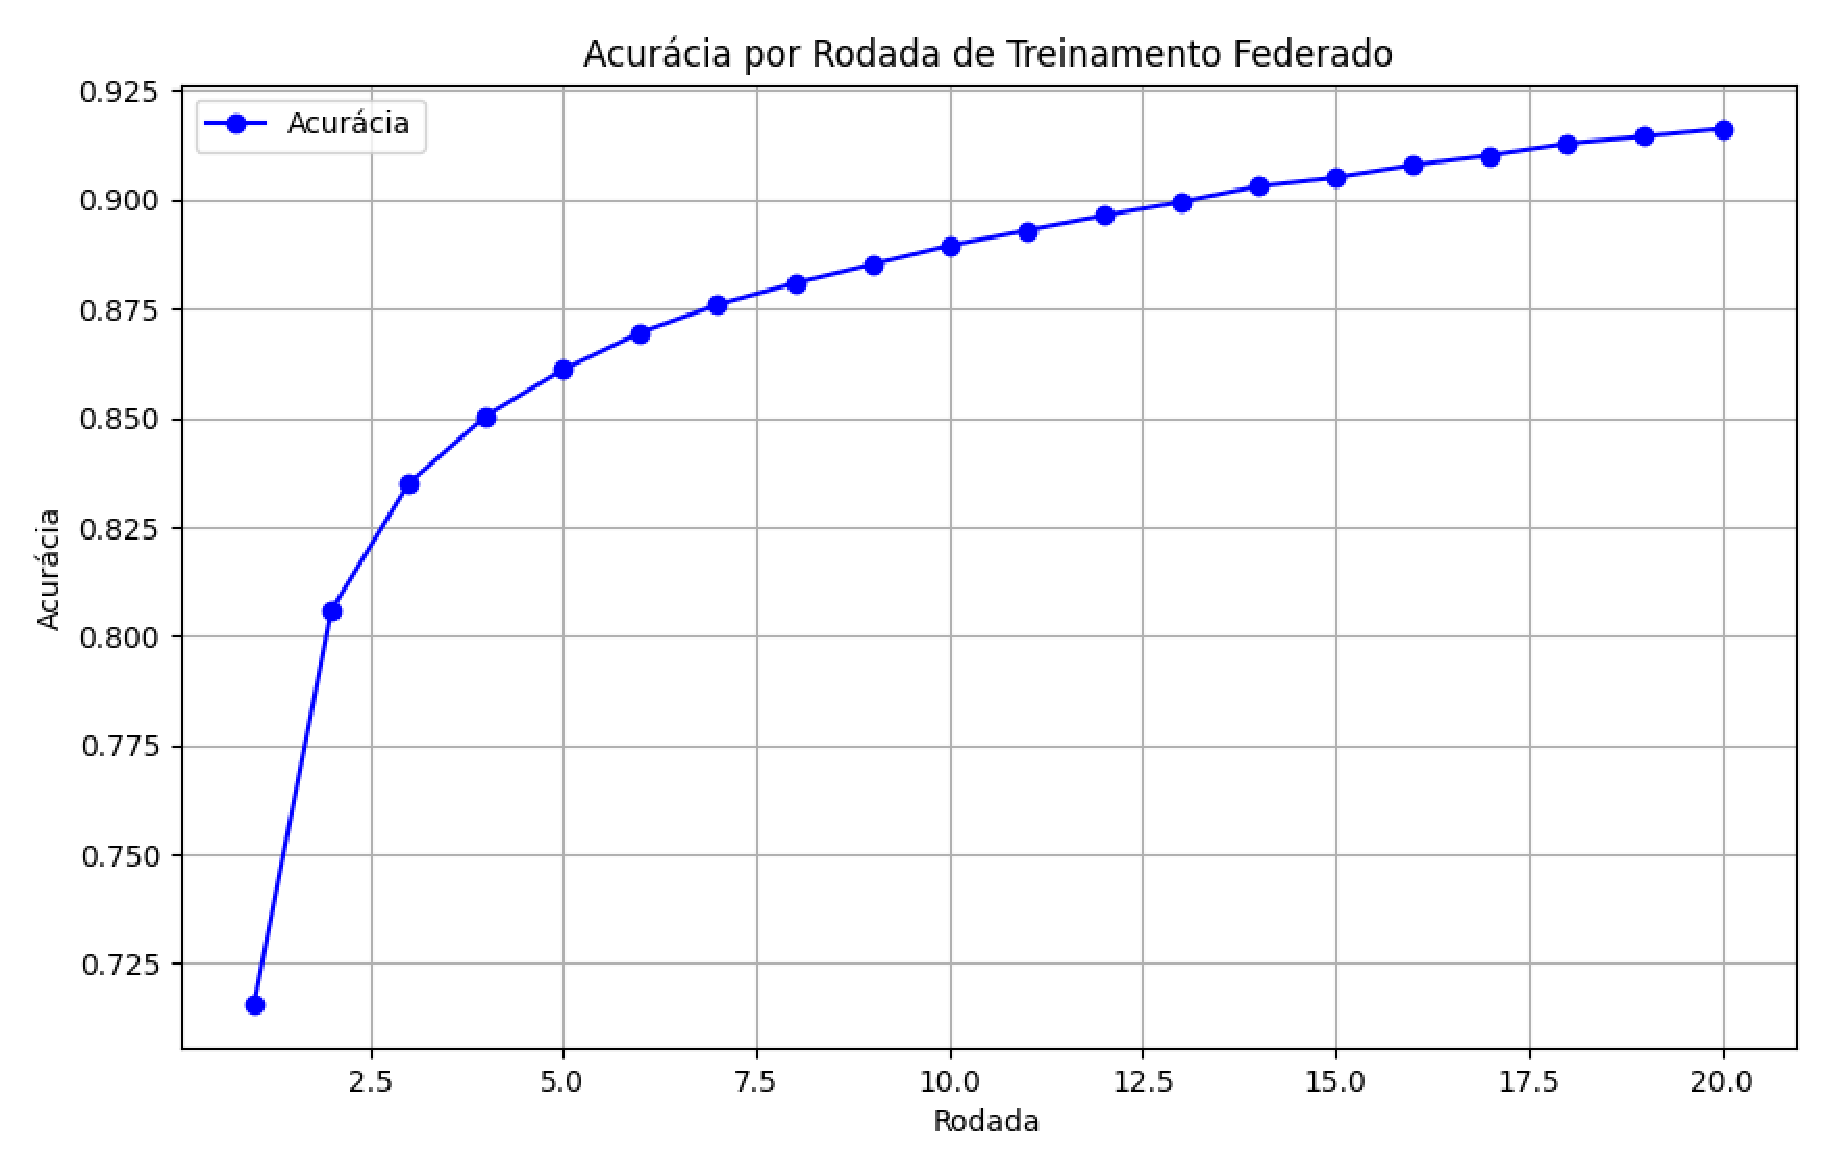
\includegraphics[scale=0.4]{figuras/analiseResultados/acuracyFederated.eps}
    \label{fig:acuracyFederated}
    \fonte{Elaborado pelo autor.}
\end{figure}

O gráfico de acurácia mostra uma evolução constante ao longo das rodadas. Na primeira rodada, o modelo federado obteve uma acurácia de aproximadamente \textbf{92,57\%}. Já na décima rodada, o modelo alcançou uma acurácia de \textbf{99,68\%}, indicando que o modelo aprendeu de forma eficaz ao longo do processo federado, conseguindo generalizar bem mesmo com os dados distribuídos.

\subsection{Acurácia \textit{Top-3}}

\begin{figure}[ht]
    \centering
    \caption{Curvas de acurácia \textit{Top-3} do modelo federado}
    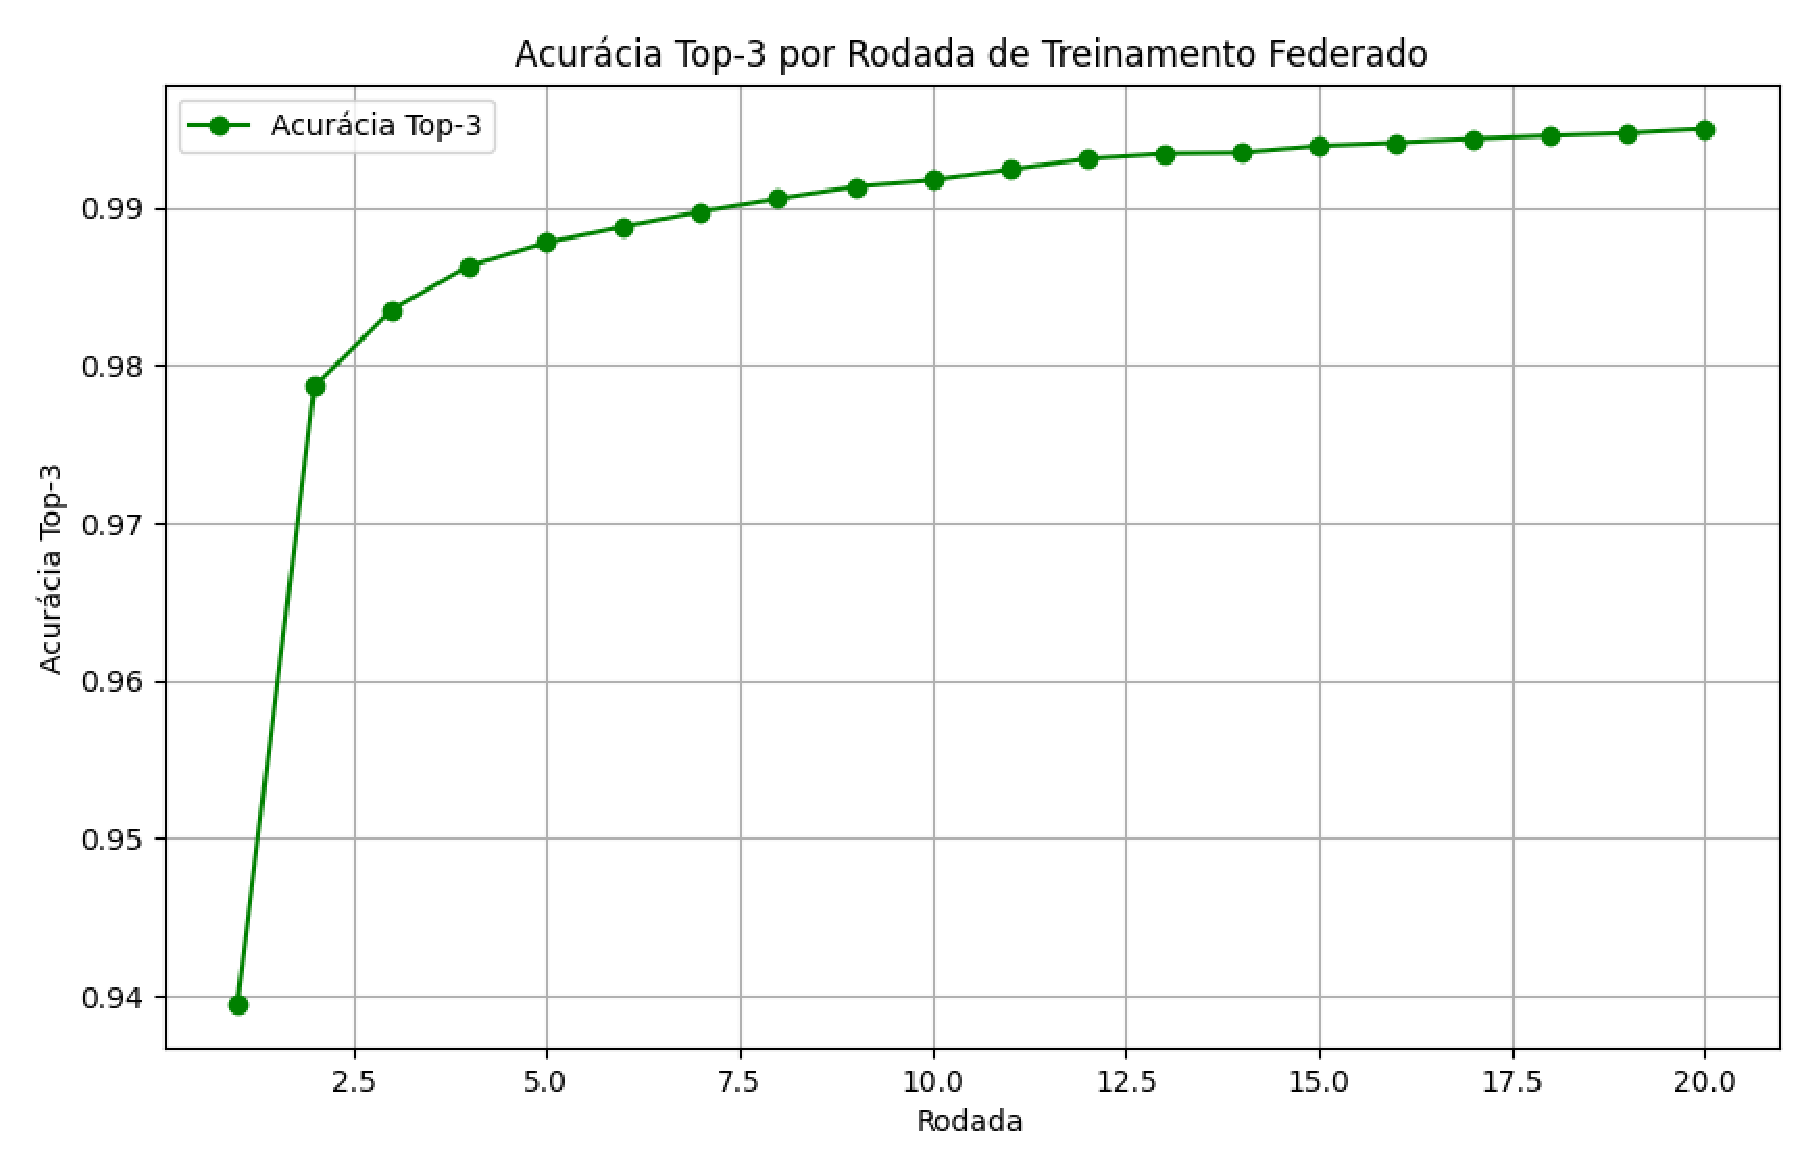
\includegraphics[scale=0.4]{figuras/analiseResultados/acuracyTop3Federated.eps}
    \label{fig:acuracyTop3Federated}
    \fonte{Elaborado pelo autor.}
\end{figure}

A acurácia \textit{Top-3}, que mede se a classe correta está entre as três previsões com maior probabilidade, começou com \textbf{98,35\%} na primeira rodada e atingiu \textbf{99,99\%} na última rodada. Isso demonstra que o modelo foi altamente eficiente ao classificar as imagens, mantendo uma alta probabilidade de acerto nas três primeiras previsões.

\subsection{Perda por Rodada}

\begin{figure}[ht]
    \centering
    \caption{Curvas de perda do modelo federado}
    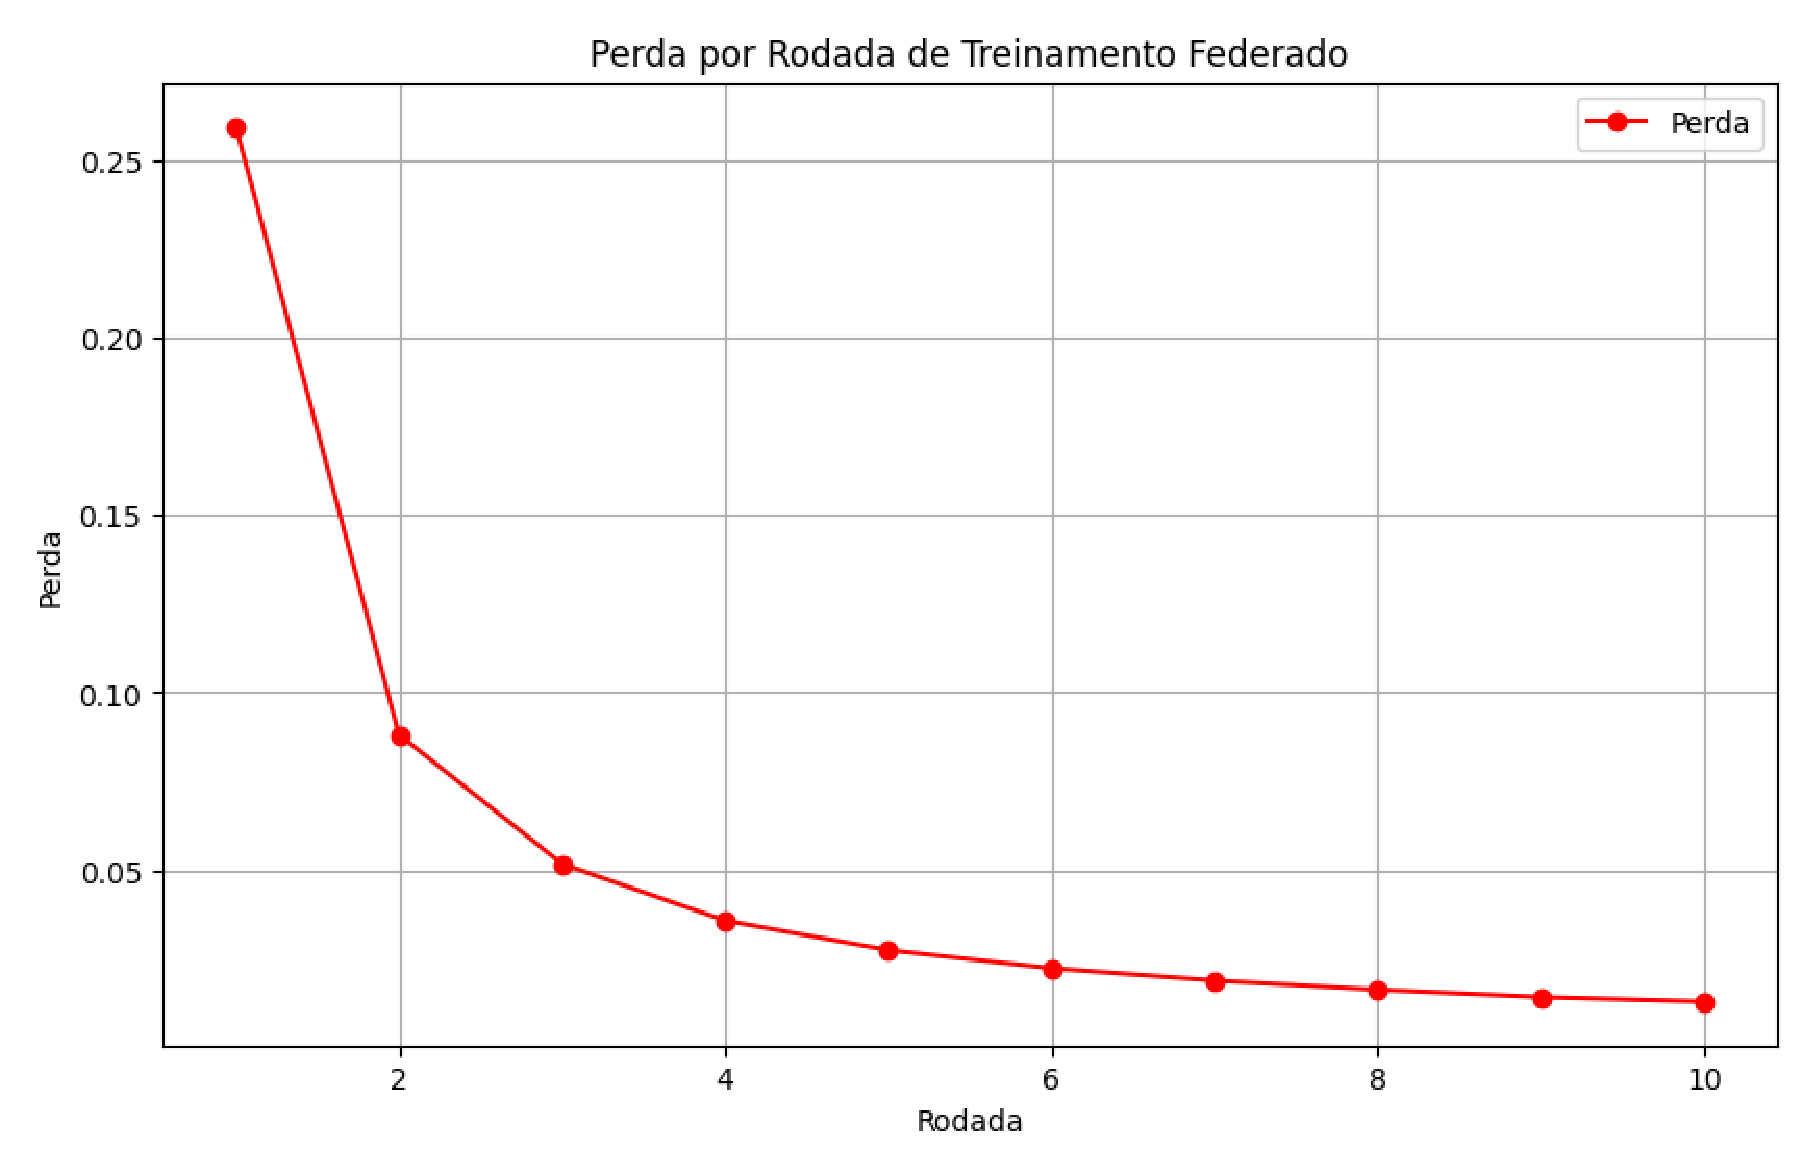
\includegraphics[scale=0.4]{figuras/analiseResultados/lossFederated.eps}
    \label{fig:lossFederated}
    \fonte{Elaborado pelo autor.}
\end{figure}

A perda no treinamento também apresentou uma redução significativa ao longo das rodadas. Iniciando com uma perda de \textbf{0,259} na primeira rodada, a perda caiu para \textbf{0,013} na décima rodada, indicando que o modelo conseguiu minimizar o erro de classificação conforme o treinamento avançou.

\subsection{Tempo de Treinamento}

O tempo total de treinamento federado foi de \textbf{4314 segundos} (aproximadamente \textbf{1 hora e 12 minutos}). Esse tempo reflete o processo de agregação e distribuição das atualizações entre os clientes e o servidor, o que é típico em ambientes de aprendizado federado, especialmente ao utilizar um grande número de clientes e iterações.

\section{Desempenho entre os Modelos}

Nesta seção, analisamos o desempenho dos modelos centralizados e federados aplicados ao conjunto de dados MNIST. As métricas de avaliação utilizadas incluem acurácia, acurácia \textit{Top-3} e perda. A comparação entre o modelo de aprendizado federado e os modelos centralizados oferece insights valiosos sobre a eficácia e a eficiência das diferentes abordagens.

\subsection{Acurácia}

A acurácia é uma métrica fundamental que indica a proporção de previsões corretas feitas pelo modelo em relação ao total de previsões. Para o modelo centralizado de MLP, a acurácia de teste alcançou \textbf{97,67\%}, enquanto o modelo DNN obteve \textbf{97,60\%}. Esses resultados demonstram que ambos os modelos centralizados foram eficazes na classificação das imagens da base MNIST, com o MLP apresentando uma ligeira vantagem.

\begin{figure}[ht]
    \centering
    \caption{Comparação de acurácia entre os modelos centralizados e federados}
    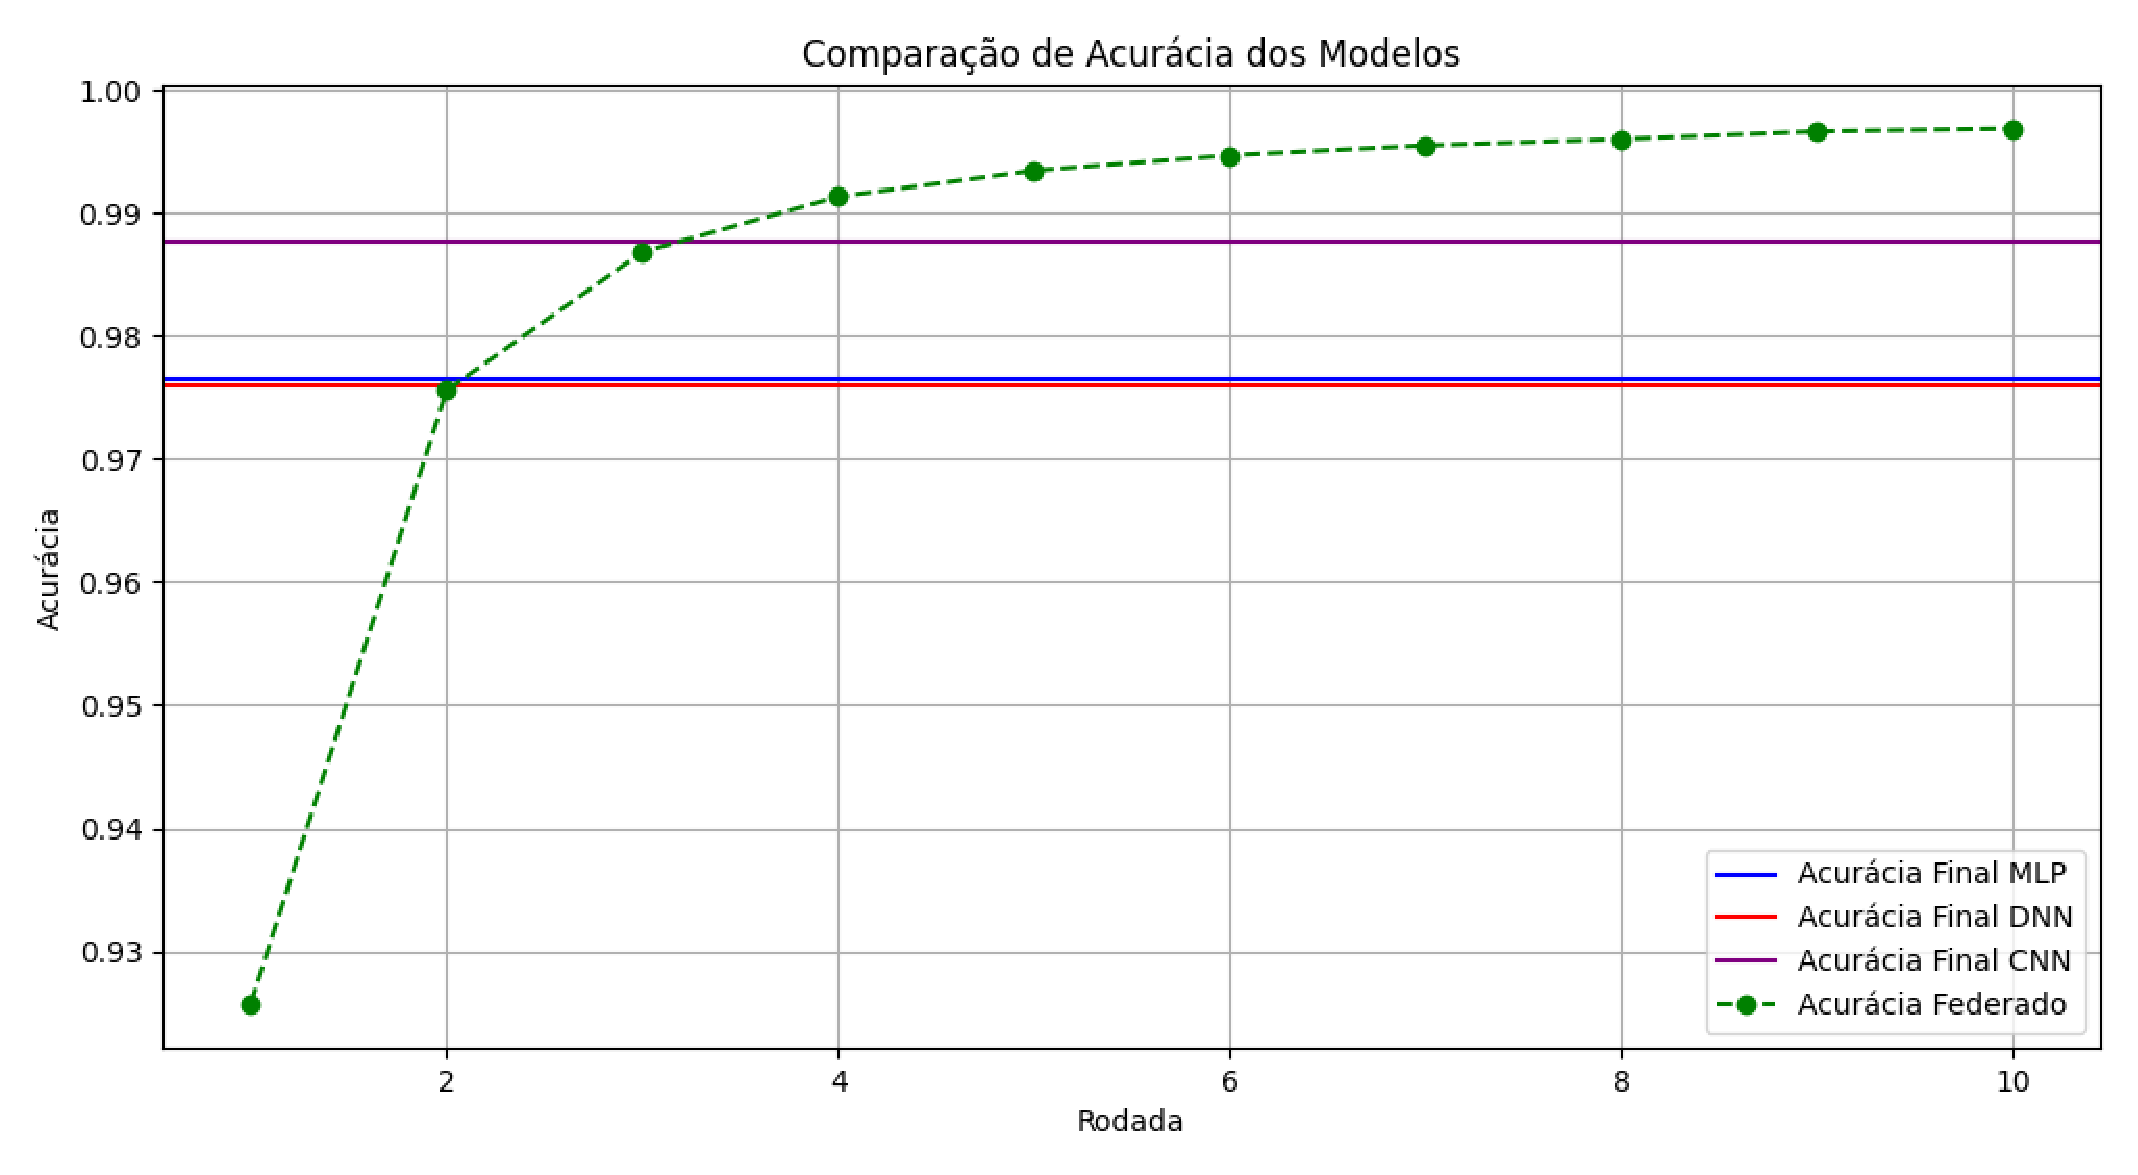
\includegraphics[scale=0.4]{figuras/analiseResultados/acuracyComparison.eps}
    \label{fig:acuracyComparison}
    \fonte{Elaborado pelo autor.}
\end{figure}

Por outro lado, o modelo federado, após 10 rodadas de treinamento, alcançou uma acurácia impressionante de \textbf{99,68\%}. Este resultado não apenas supera os modelos centralizados, mas também indica uma excelente capacidade de generalização do modelo federado, mesmo com os dados distribuídos entre múltiplos clientes. A expectativa pré-treinamento era de que o modelo federado pudesse oferecer desempenho competitivo, mas a acurácia obtida ultrapassou as expectativas, sugerindo que o aprendizado federado é uma abordagem viável e eficiente para preservação da privacidade sem comprometer a precisão do modelo.

\subsection{Acurácia \textit{Top-3}}

A acurácia \textit{Top-3} é uma métrica adicional que mede a proporção de vezes em que a classe correta está entre as três principais previsões do modelo. Essa métrica é particularmente útil para avaliar a confiabilidade do modelo em cenários onde uma única previsão pode não ser suficiente. No treinamento centralizado, a acurácia \textit{Top-3} não foi diretamente medida para os modelos MLP e DNN. No entanto, para o modelo federado, a acurácia \textit{Top-3} começou em \textbf{98,35\%} e atingiu \textbf{99,99\%} após 10 rodadas.

Este desempenho notável do modelo federado na métrica \textit{Top-3} reforça a sua eficácia não apenas em fazer previsões corretas, mas também em fornecer previsões confiáveis entre as três opções mais prováveis. A melhoria constante observada ao longo das rodadas de treinamento sugere que o modelo federado consegue refinar suas previsões de forma eficiente, mesmo em um ambiente descentralizado. Isso é um indicativo de que o modelo é robusto e confiável, mantendo uma alta probabilidade de incluir a resposta correta nas suas três principais previsões.

\subsection{Perda}

A perda é uma métrica que quantifica a discrepância entre as previsões do modelo e os valores reais, representando a eficácia do modelo em minimizar erros durante o treinamento. Para o modelo MLP, a perda de teste foi de \textbf{0,1013}, e para o modelo DNN foi de \textbf{0,1101}. Ambos os modelos centralizados mostraram desempenhos bastante similares em termos de perda, com o MLP ligeiramente superior.

\begin{figure}[ht]
    \centering
    \caption{Comparação de perda entre os modelos centralizados e federados}
    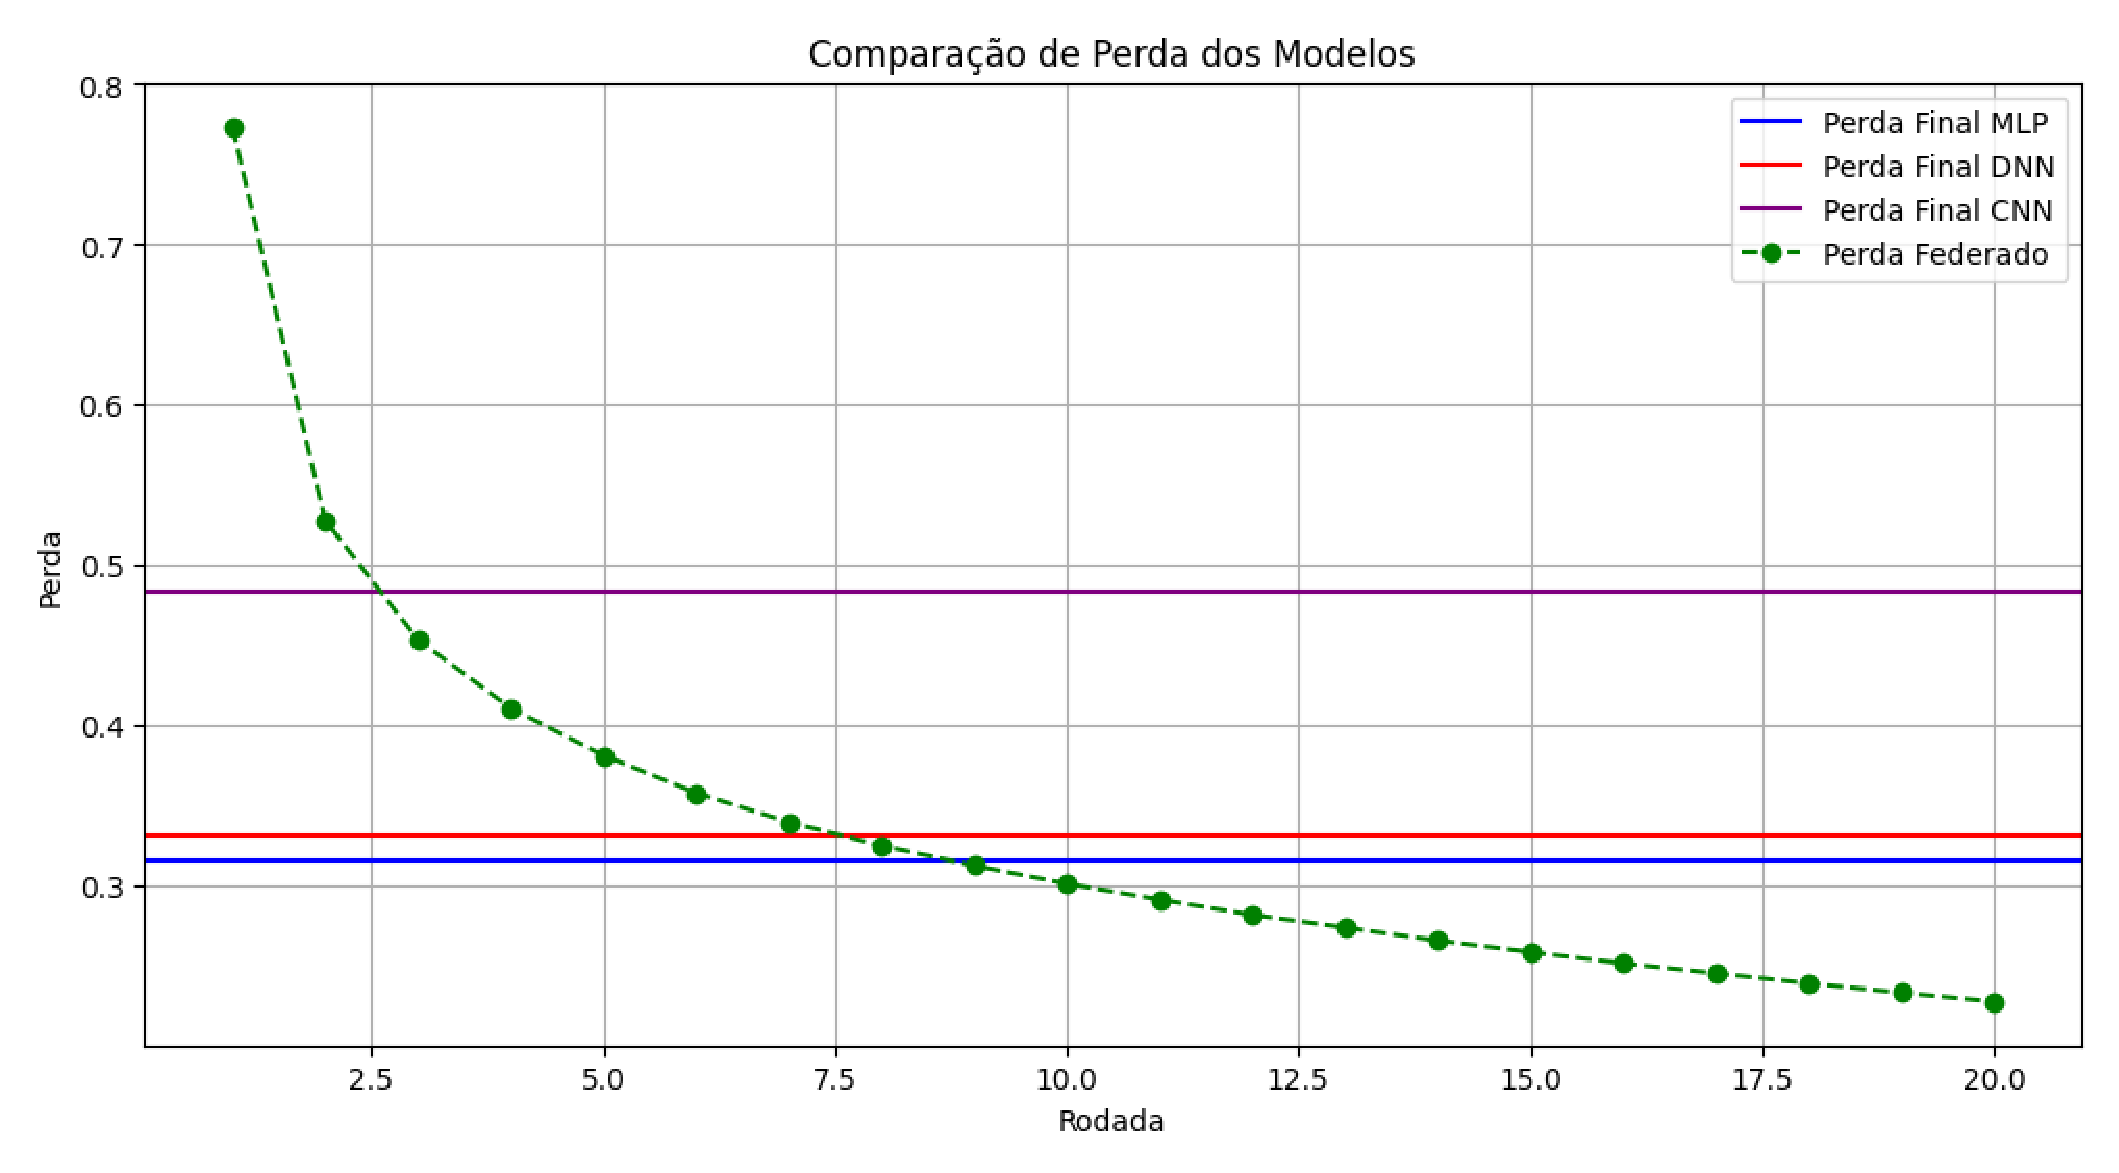
\includegraphics[scale=0.4]{figuras/analiseResultados/lossComparison.eps}
    \label{fig:lossComparison}
    \fonte{Elaborado pelo autor.}
\end{figure}

O modelo federado, por sua vez, iniciou com uma perda de \textbf{0,259} na primeira rodada e conseguiu reduzir essa métrica para \textbf{0,013} ao final das 10 rodadas. A significativa redução na perda ao longo do treinamento federado demonstra que o modelo federado foi capaz de aprender e ajustar seus parâmetros de forma eficaz, minimizando os erros de classificação. Essa tendência de diminuição da perda indica que o modelo federado não apenas tem uma acurácia alta, mas também é eficaz em ajustar suas previsões para se alinhar mais de perto com os valores reais, o que é um resultado positivo considerando o cenário de aprendizado distribuído.

\section{Considerações Finais}

A comparação entre o modelo federado e os modelos centralizados revela que o aprendizado federado pode alcançar, e até superar, o desempenho dos modelos centralizados em termos de acurácia, acurácia \textit{Top-3} e perda. As expectativas pré-treinamento de que o modelo federado poderia oferecer desempenho competitivo foram confirmadas e, em muitos aspectos, superadas. Esses resultados demonstram que o aprendizado federado é uma abordagem poderosa e eficiente para treinamento de modelos de IA, permitindo a preservação da privacidade dos dados sem sacrificar a precisão e a eficácia do modelo. A análise detalhada das métricas reforça a viabilidade e a vantagem do aprendizado federado em ambientes onde a privacidade dos dados é crucial.

\section{Dificuldades e Limitações}

A seção de dificuldades e limitações explora os desafios enfrentados durante o desenvolvimento dos modelos de aprendizado centralizado e federado, as influências dessas dificuldades na escolha da base de dados e as implicações do uso do Google Colab no treinamento dos modelos. Esta análise fornece uma visão crítica sobre as limitações dos métodos de treinamento e os aspectos técnicos que impactaram o progresso e os resultados do projeto.

\subsection{Dificuldades no Desenvolvimento dos Modelos}

Desenvolver modelos de aprendizado centralizado e federado envolveu uma série de desafios técnicos e conceituais. Para os modelos centralizados, como o MLP e o DNN, uma das principais dificuldades foi o ajuste dos hiperparâmetros, como a taxa de aprendizado e o número de camadas e neurônios. A escolha inadequada desses parâmetros pode levar a problemas como overfitting ou underfitting, impactando negativamente a precisão e a capacidade de generalização dos modelos. Além disso, a gestão do treinamento e a monitorização das métricas de desempenho foram essenciais para garantir que o modelo estivesse aprendendo de forma eficaz e não estivesse simplesmente decorando os dados de treinamento.

\subsection{Influência na Escolha da Base de Dados}

A escolha da base de dados MNIST foi fortemente influenciada pelas limitações e dificuldades enfrentadas. MNIST é uma base de dados relativamente simples e bem compreendida, o que a torna ideal para testar e validar conceitos iniciais de aprendizado de máquina e federado. A simplicidade do MNIST permite a implementação e o ajuste dos modelos sem a complexidade adicional que outras bases de dados mais desafiadoras poderiam introduzir. O uso de MNIST facilitou a identificação de problemas e a realização de ajustes nos modelos, sem o impacto adicional das complexidades associadas a bases de dados mais sofisticadas.

No entanto, a simplicidade do MNIST também significa que as dificuldades enfrentadas no desenvolvimento dos modelos podem não refletir os desafios encontrados em cenários mais complexos e realistas. Modelos treinados com MNIST podem não se comportar da mesma forma quando aplicados a bases de dados mais complexas ou em cenários reais de aprendizado federado, onde a heterogeneidade dos dados e a comunicação entre clientes podem ser mais desafiadoras.

\subsection{Impacto do Google Colab no Treinamento dos Modelos}

O uso do Google Colab teve um impacto significativo no desenvolvimento e no treinamento dos modelos. Google Colab fornece uma plataforma acessível e com recursos computacionais relativamente poderosos, como GPUs, o que facilitou o treinamento dos modelos, especialmente para o modelo DNN que exige maior capacidade computacional. No entanto, existem limitações associadas ao uso de Google Colab, como restrições de tempo de execução e limitações de memória. Essas restrições podem impactar o treinamento de modelos mais complexos ou o uso de grandes conjuntos de dados.

\subsection{Limitações dos Métodos de Treinamento}

Os métodos de treinamento centralizado e federado apresentam suas próprias limitações. No treinamento centralizado, um desafio é a necessidade de grandes volumes de dados e poder computacional para alcançar resultados precisos e generalizáveis. Modelos mais complexos podem exigir ajustes finos e otimização que podem não ser práticos em todas as situações. Além disso, o treinamento centralizado não aborda diretamente a questão da privacidade dos dados, o que pode ser uma limitação significativa em contextos onde a proteção da privacidade é essencial.

Por outro lado, o aprendizado federado, embora ofereça vantagens significativas em termos de privacidade e segurança dos dados, enfrenta limitações relacionadas à comunicação e sincronização entre os clientes. A agregação de modelos locais pode ser influenciada pela heterogeneidade dos dados e pelas condições variáveis de treinamento nos diferentes clientes. Além disso, o custo computacional e a complexidade do protocolo de treinamento federado podem ser desafiadores, especialmente quando se lida com um grande número de clientes e uma vasta quantidade de dados.